\chapter{Clasificatori}

Clasificatorii, în învățarea automată, reprezintă algoritmi care, pe baza unor seturi de date de diferite tipuri,
pot prezice tipurile unor date noi, pe care algoritmul "nu le-a văzut". În continuare voi prezenta clasficatorii
folosiți de mine. Toți algoritmii folosiți sunt din biblioteca scikit-learn, din Python.

\section{SVC}

SVC (Support Vector Classifier) este un clasificator cu o idee de bază simplă și elegantă. Acesta, în combinație
cu SVM (Support Vector Machine), clasifică datele printr-un hiperplan într-un hiperspațiu (mai mare decât cel format caracteristicile datelor).
De exemplu, există posibilitatea ca două seturi de puncte să nu poată fi despărțite de un singur hiperplan, în hiperspațiul definit de caracteristici,
iar pentru a rezolva această problemă, prin intermediul unei funcții nucleu (polinomială sau rbf), se proiectează punctele într-un 
hiperspațiu superior, acestea putând fi clasificate de către un hiperplan.

Hipeplanul separator definit de acest clasificator se bazează pe găsirea unei margini maxime, dar care să nu ia în considerare
punctele de tip "outlier", această margine numindu-se "moale" (soft margin). Pentru a realiza acest lucru, se face o antrenare de tip
cross-validation, după care se alege cea mai bună margine.

Aceste funcții nu proiectează propriu-zis punctele într-un hiperplan superior, ci calculează relația acestora în hiperplanul respectiv.
Funcția polinomială, descrisă de formula \[(a \times b + r)^d\], are ca parametru \(d\), care reprezintă dimensiunea proiecției, \(r\) 
este o constantă, iar \(a\) și \(b\) sunt coordonatele punctelor, adică vectorii elementelor pentru care se dorește calcularea relației.
Această funcție este limitată la un număr finit de dimensiuni.

Rbf este o funcție mai complexă, aceasta nefiind limitată de numărul de dimensiuni, calculul acesteia reprezentând un hiperspațiu infinit.
Este definită de formula \[e^{-\gamma (a - b) ^ {2}}\], în care \(a\) și \(b\) reprezintă același lucru (vectorii pentru care se calculează relația), iar
\(\gamma\) este o constantă.

În continuare vom demonstra că funcția rbf se poate scrie ca un produs infinit. Pentru început, alegem \(\gamma = \frac{1}{2}\), iar funcția va deveni:
\[e^{-\frac{1}{2} (a - b) ^ {2}} = e^{-\frac{1}{2}(a^2 + b^2) + \frac{1}{2}2ab} = e^{-\frac{1}{2}(a^2 + b^2)} \cdot e^{ab}\] .
Următorul pas este aproximarea funcției \(e^{ab}\) cu o serie Taylor, cu a = 0. Fie următoarea serie pentru \(e^x\), ținându-se cont de faptul că derivatele acesteia sunt egale cu funcția exponențială:
\[e^x = e^0 + e^0 \cdot x + \frac{e^0}{2!}x + \frac{e^0}{3!}x^2 + \dotsb + \frac{e^0}{n!}x^n + \dotsb\]
Înlocuim \(x\) cu \(ab\), iar ecuația devine:
\[e^{ab} = 1 + ab + \frac{1}{2!}(ab)^2 + \frac{1}{3!}(ab)^3 + \dotsb + \frac{1}{n!}(ab)^n + \dotsb\], care poate fi scrisă:
\[e^{ab} = (1, a, \frac{1}{\sqrt{2!}}a^2, \frac{1}{\sqrt{3!}}a^3, \dotsb, \frac{1}{\sqrt{n!}}a^n, \dotsb) \cdot (1, b, \frac{1}{\sqrt{2!}}b^2, \frac{1}{\sqrt{3!}}b^3, \dotsb, \frac{1}{\sqrt{n!}}b^n, \dotsb)\]
Folosind notația \(e^-\frac{1}{2}(a^2 + b^2) = s\), ecuația inițială va arăta astfel:
\[e^{-\frac{1}{2} (a - b) ^ {2}} = (s, sa, \frac{1}{\sqrt{2!}}sa^2, \frac{1}{\sqrt{3!}}sa^3, \dotsb, \frac{1}{\sqrt{n!}}sa^n, \dotsb) \cdot (1, sb, \frac{1}{\sqrt{2!}}sb^2, \frac{1}{\sqrt{3!}}sb^3, \dotsb, \frac{1}{\sqrt{n!}}sb^n, \dotsb)\]
Drept urmare, am putut scrie funcția rbf ca un produs de doi vectori infiniți.

În următoarea imagine se poate observa cum se face trecerea unor puncte dintr-un spațiu 2-dimensional într-unul 3-dimensional, după care
se găsește planul despărțitor.

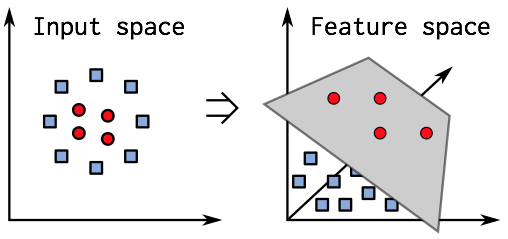
\includegraphics[width=0.8\textwidth]{svm.png.png}


Am încercat ambele funcții nucleu, însă rbf (radial basis function) a avut rezultate mai bune. Diferența între cele două este că
funcția rbf proiectează punctele într-un hiperplan infinit, folosindu-se de o aproximare Taylor (serie Taylor), iar cea polinomială 
le proiectează într-un hiperspațiu de dimensiune n.


Acesta a fost clasificatorul care a obținut cele mai bune rezultate, însă a fost mai lent decât ceilalți.


\section{Rețea neuronală}

Am încercat antrenarea și cu o rețea neuronală, folosind biblioteca keras, însă nu prea am avut rezultate bune. Am încercat mai multe
structuri (1, 2, 3 straturi ascunse), diferite funcții de activare pe ultimul strat, pentru straturile din interior folosind funcția RELU,
diferiți opimiziatori (adam, SGD, etc.). Configurația optimă este alcătuită din 2 staturi interioare, de 80 și respectiv 20 de neuroni, optimizatorul adam,
funcția de cost crosentropie binară și funcția de activare de pe ultimul strat sigmoid. Această configurație a produs un f-score de 0.12, care
este foarte slab. Numărul de epoci l-am ținut cât mai mic, deoarece face overfit foarte rapid, în această problemă fiind nevoie de găsirea unor 
caracteristici mai generale.

Pentru realizarea unor comparații între mai multe configurații ale rețelei, am folosit situl \href{https://app.wandb.ai/}{wandb}.

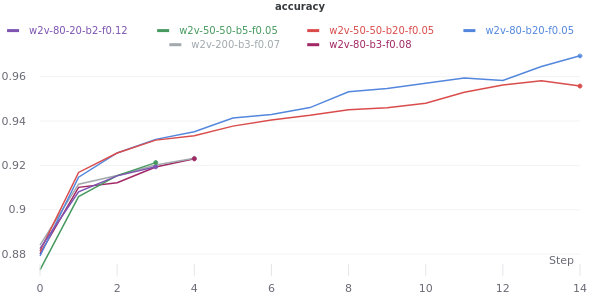
\includegraphics[width=0.4\textwidth]{w2v-acc.png}
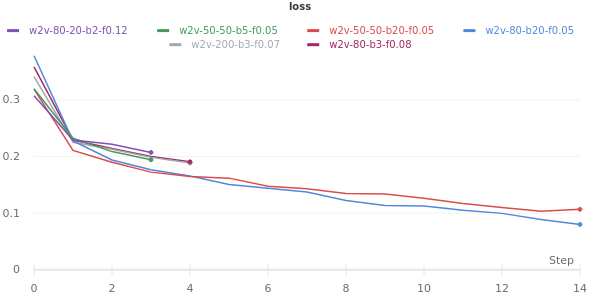
\includegraphics[width=0.4\textwidth]{w2v-loss.png}

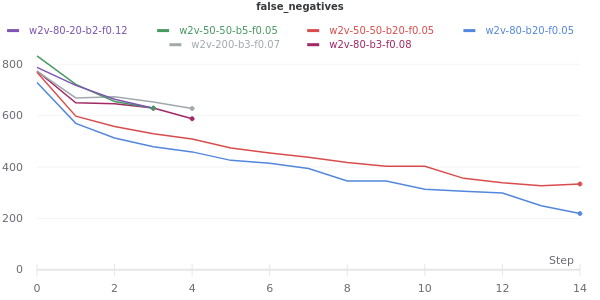
\includegraphics[width=0.4\textwidth]{w2v-fn.png}
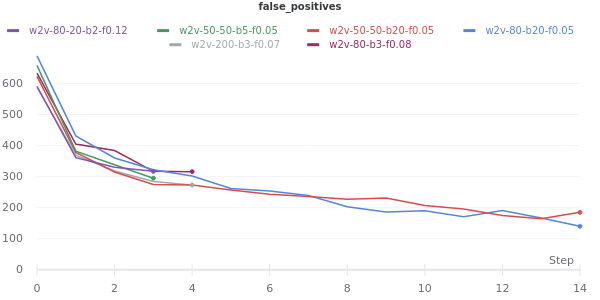
\includegraphics[width=0.4\textwidth]{w2v-fp.png}

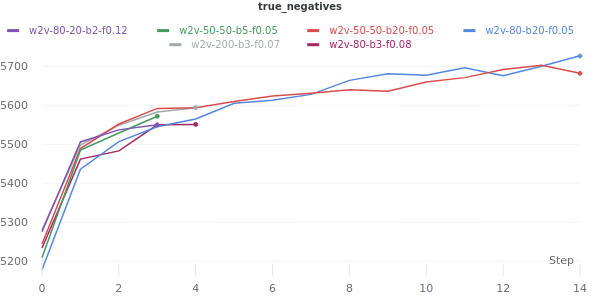
\includegraphics[width=0.4\textwidth]{w2v-tn.png}
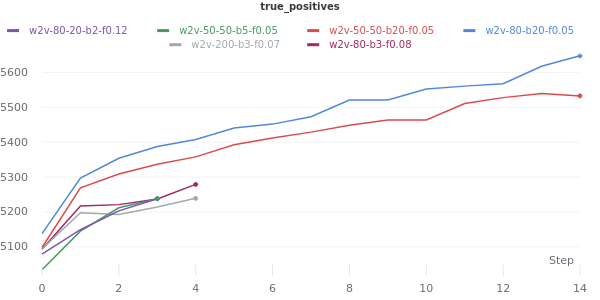
\includegraphics[width=0.4\textwidth]{w2v-tp.png}

După cum se vede în aceste grafice, rețeaua neuronală are cam aceeași direcție.


\section{Bayes Naiv}

În încercarea de a găsi un clasificator mai bun decât SVC, am vrut să aleg ceva simplu, care nu e predispus la overfitting, și 
știam că metoda Bayes Naiv respectă aceste lucruri. Acesta se bazează pe formula lui Bayes, însă face o presupunere puternică, și
aceea că proprietățile sunt independente. Acest lucru face și timpul de antrenare mult mai mic deoarece, având variablile independente,
formula lui Bayes devine un produs al probabilităților fiecărei caracteristici.

Folosind această metodă, am obținut rezultate chiar bune, puțin mai slabe decât ale clasificatorului SVC, însă mult mai rapid decât acesta.

\section{Regresie Logistică}

În ciuda numelui, regresia logistică este un algoritm de clasificare, nu de regresie. Denumirea acestei metode vine de la funcția logistică (sigmoidă)
care stă la bază. Deoarece calculează probabilitatea ca o intrare să fie de un anumit tip, acest algoritm este bun pentru o clasificare binară.
El se bazează pe folosirea funcții sigmoide, pentru a calcula probabilitatea menționată.

În exemplul de mai jos, se observă curba determinată de funcția logistică.

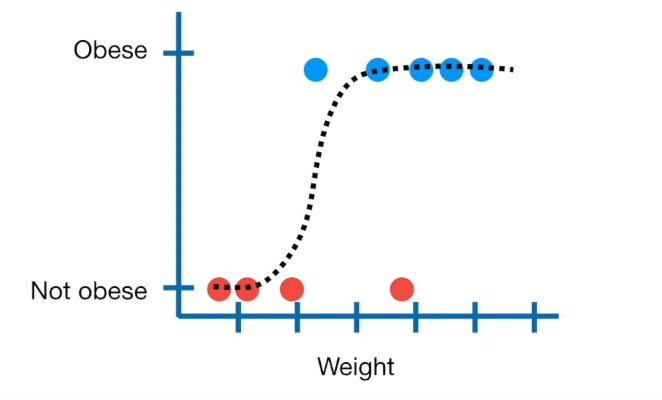
\includegraphics{logistic.jpg}

Antrenarea acestui clasificator constă în aproximarea coeficienților funcției, folosind MLE (Maximum Likelihood Estimation).
Formula de mai jos reprezintă un exemplu de ecuație logistică: \[y = \frac{e^{b_0 + b_{1} \cdot x}}{1 + e^{b_0 + b_{1} \cdot x}}\],
unde \(y\) reprezintă outputul prezis, \(b_0\) reprezintă bias-ul, iar \(b_1\) este coeficientul pentru o intrare \(x\). Pentru fiecare coloană
(caracteristică) există un coeficient \(b\), care trebuie învățat din setul de antrenare.

Această metodă calculează probabilitatea ca o intrarea \(x\) să fie de o clasă \(y\), prestabilită, după formula 
\[P(X) = P(Y=1|X)\]
Această probabilitate va fi comparată cu un prag, de obicei 0.5, după care se va stabili clasa vectorului respectiv.
Regresia logistică este o metodă liniară, dar predicțiile sunt transformate folosind funcția logistică. Impactul acestei metode 
este că nu mai putem înțelege prezicerile ca o combinație liniară a inputurilor, ca în cazul regresiei liniare, de exemplu. În continuare,
modelul poate fi descris de formula:
\[p(X) = \frac{e^{b_0 + b_1 X}}{1 + e^{b_0 + b_1 X}}\]
Logaritmând, obținem:
\[ln(p(X)) = b_0 + b_1 X - ln(1 + e^{b_0 + b_1 X})\]
\[ln(p(X)) + ln(\frac{1}{\frac{1}{1 + e^{b_0 + b_1 X}}}) = b_0 + b_1 X\]
\[ln(\frac{p(X)}{1 - \frac{e^{b_0 + b_1 X}}{1 + e^{b_0 + b_1 X}}}) = b_0 + b_1 X\]
\[ln(\frac{p(X)}{1 - p(X)}) = b_0 + b_1 X\]
Ecuația a devenit din nou liniară, iar raportul din stânga reprezintă șansele.
\[ln(odds) = b_0 + b_1 X\], după care exponențiem, și obținem:
\[odds = e^{b_0 + b_1X}\]
Asta arată că, chiar dacă este neliniară, pleacă de la liniaritatea log-șanselor.


Rezultatele acestei metode au fost mai bune decât ale Bayesului Naive, dar mai slabe decât ale SVC-ului.




